\documentclass{article}

\usepackage{float}
\usepackage{geometry}
\usepackage{graphicx}
\usepackage{pgf}
\usepackage{tikz}

\geometry{margin=1in}

\graphicspath{ {figures/}{photos/} }

\usetikzlibrary{arrows}
\usetikzlibrary{automata}
\usetikzlibrary{fit}
\usetikzlibrary{positioning}
\tikzset{initial text={}}

\title{Report: Room Detector}
\author{Jeremiah Griffin}
\date{Spring 2017}

\begin{document}

\pagenumbering{gobble}
\maketitle
\newpage

\pagenumbering{roman}
\tableofcontents
\listoffigures
\listoftables
\newpage

\pagenumbering{arabic}

\section{Introduction}

The room detector uses inputs from several sensors to determine what
room or environment the device is currently in.  It uses a statistical
model to associate ambient factors with a user-defined room number.  The
network must be trained by the user before it may be used.  This is done
online by placing the device in each room to be detected, entering
training mode, associating either a new or existing room number with the
training data, and then moving the device through the room.  The longer
the device is trained, the more accurate its classifications become.
Once training is complete, the device may enter detection mode and be
moved between any of the trained rooms.  If brought to an untrained
room, it will make its best guess at classifying the room as one that
was trained.

\begin{figure}[h]
  \centering
  \noindent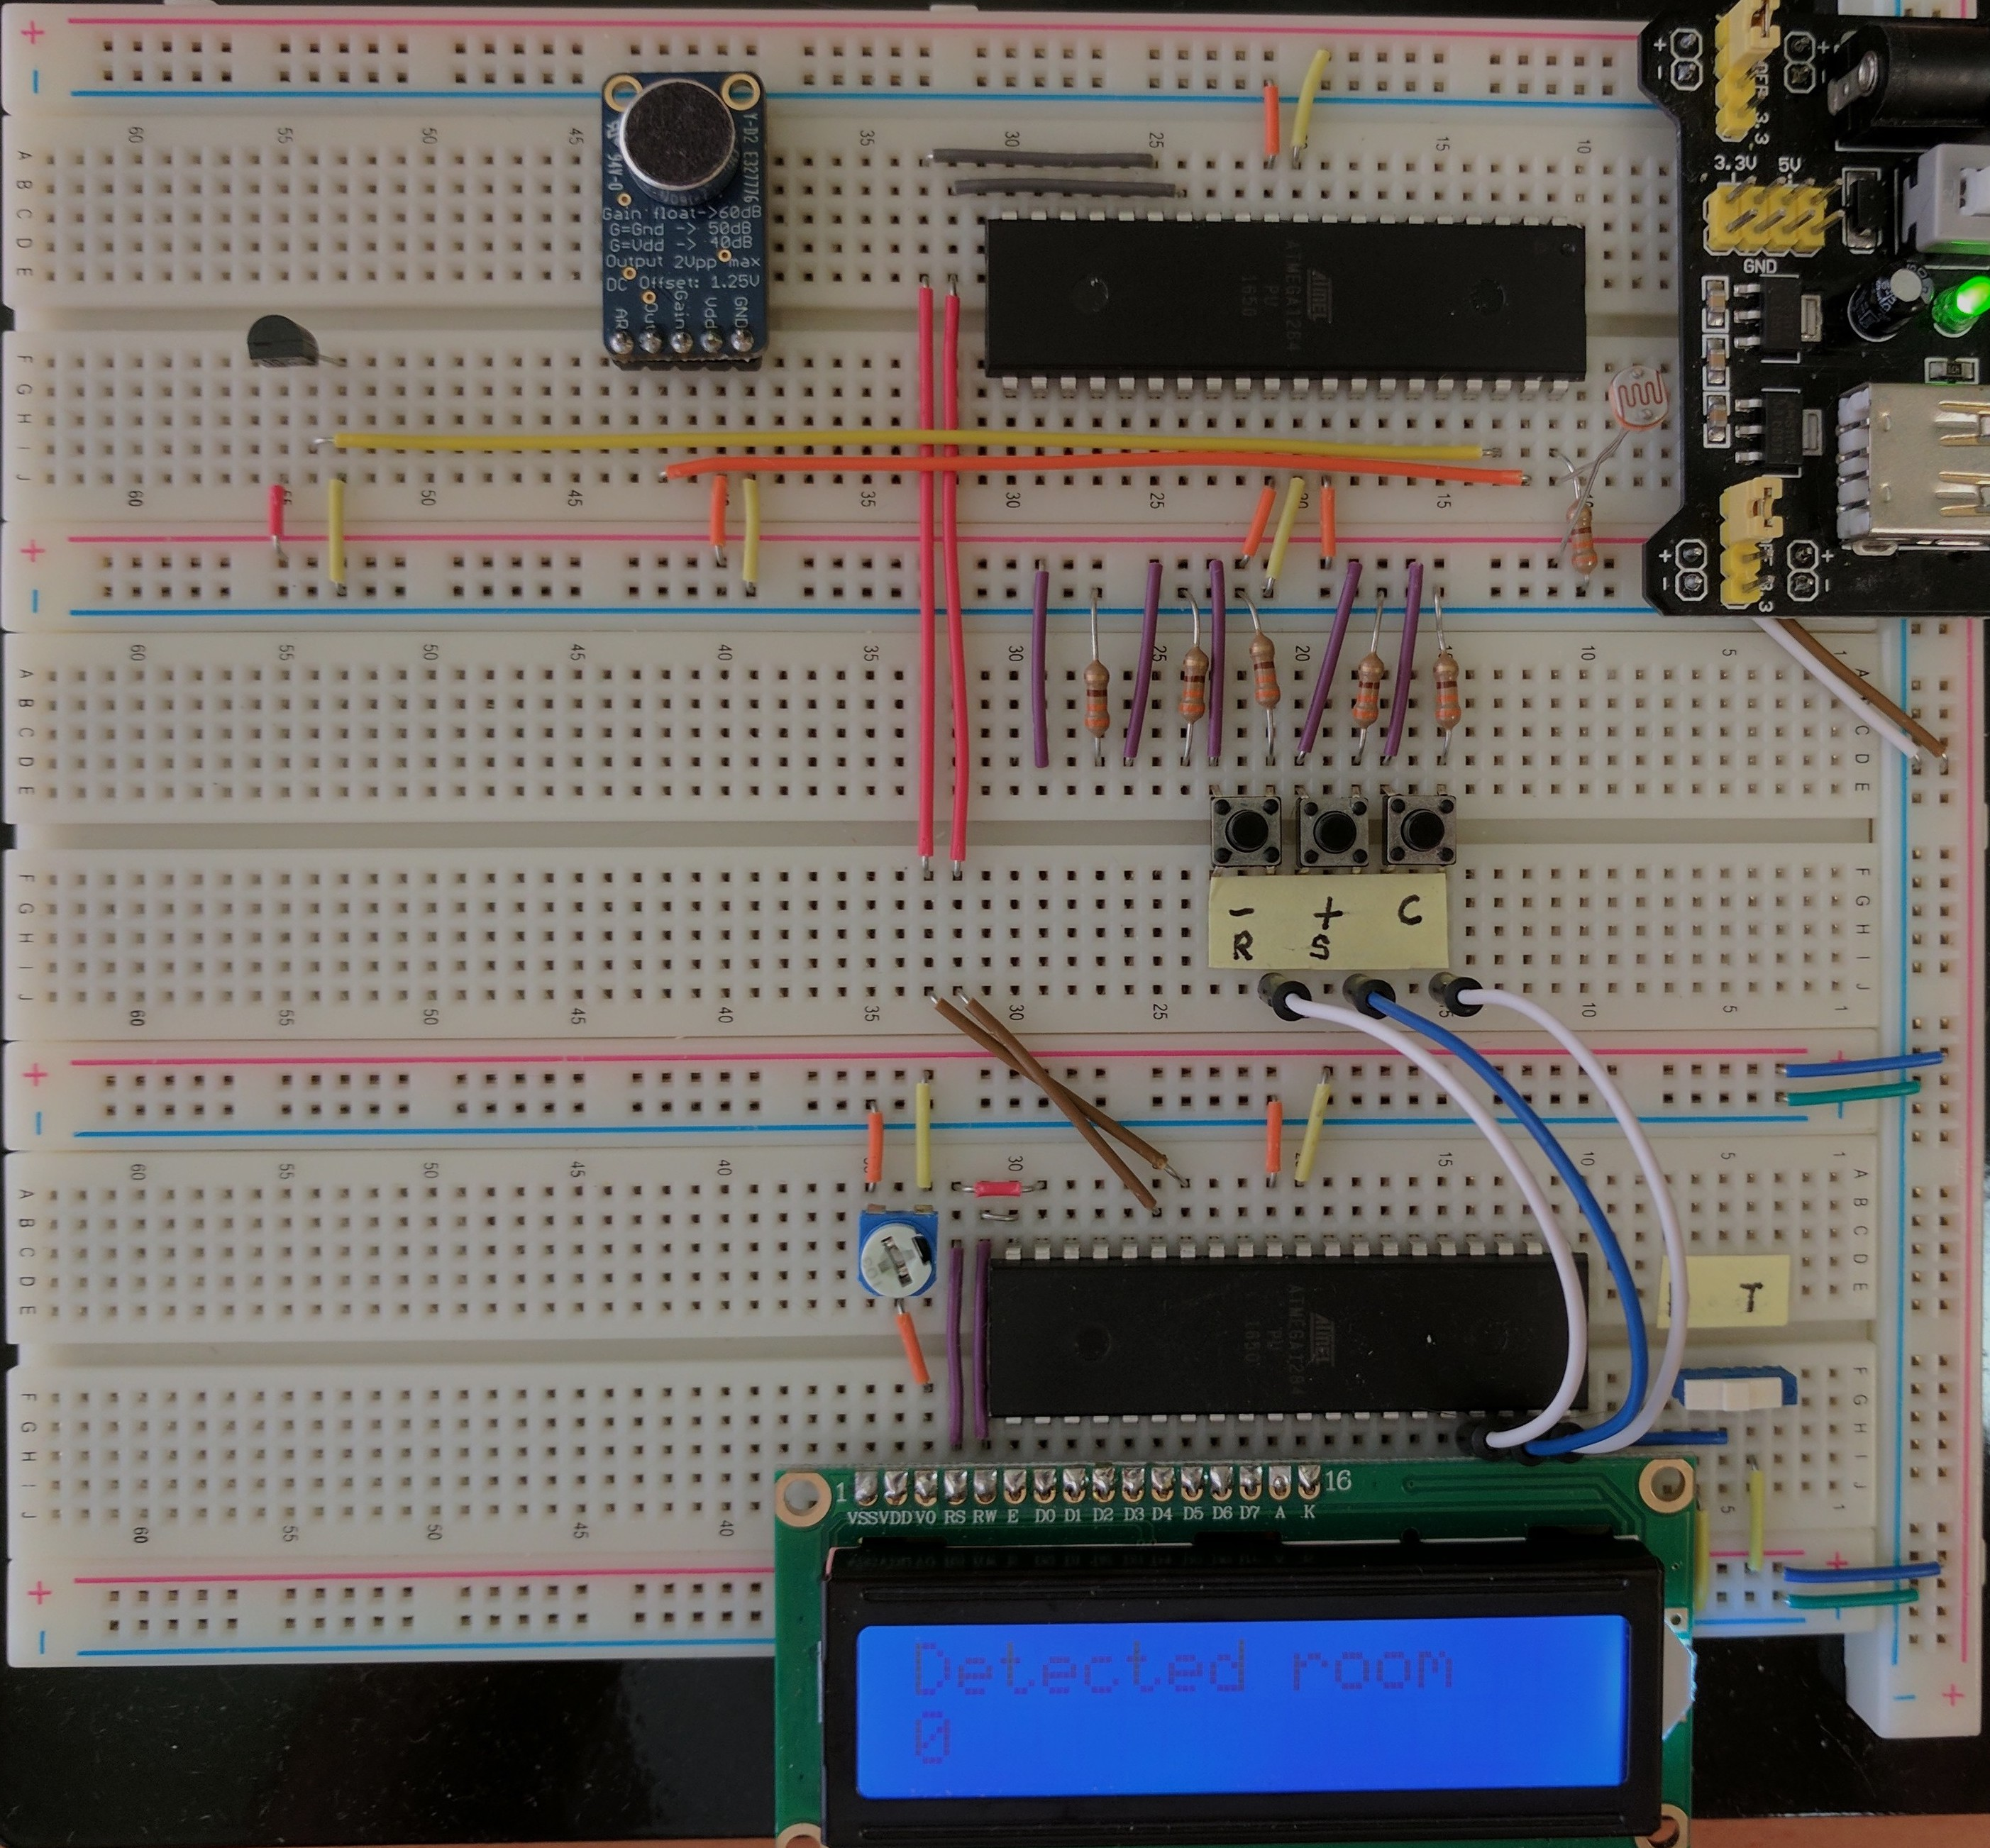
\includegraphics[width = \textwidth]{overview}
  \caption{Overview photo of project hardware}
  \label{photo:1}
\end{figure}

\section{Hardware}

\subsection{Parts}

The hardware components that were used in this project are listed below.
The equipment that was not taught as part of the course material is
listed in bold.

\begin{table}[h!]
  \centering
  \begin{tabular}{llr}
    Part Number & Component & Quantity \\
    \hline
    ATmega1284p             & Microcontroller                  & 2 \\
                            & SPDT toggle switch               & 1 \\
                            & SPST push-down button            & 3 \\
                            & 10K\Omega\ trimmer potentiometer & 1 \\
                            & 330\Omega\ 10\% resistor         & 4 \\
                            & CdS photoresistor                & 1 \\
    LCM-S01602DTR/M         & Liquid crystal display           & 1 \\
    \textbf{TMP36}          & Temperature sensor               & 1 \\
    \textbf{CMA-4544PF-W}   & Electret microphone              & 1 \\
    \textbf{MAX9814}        & Microphone amplifier             & 1
  \end{tabular}
  \caption{Listing of parts used in design}
  \label{table:1}
\end{table}

\subsection{Pinout}

\section{Software}

The software designed for this project was implemented using the PES
standard.  The overall design as a task diagram is included below.

\begin{figure}[H]
  \centering
  \noindent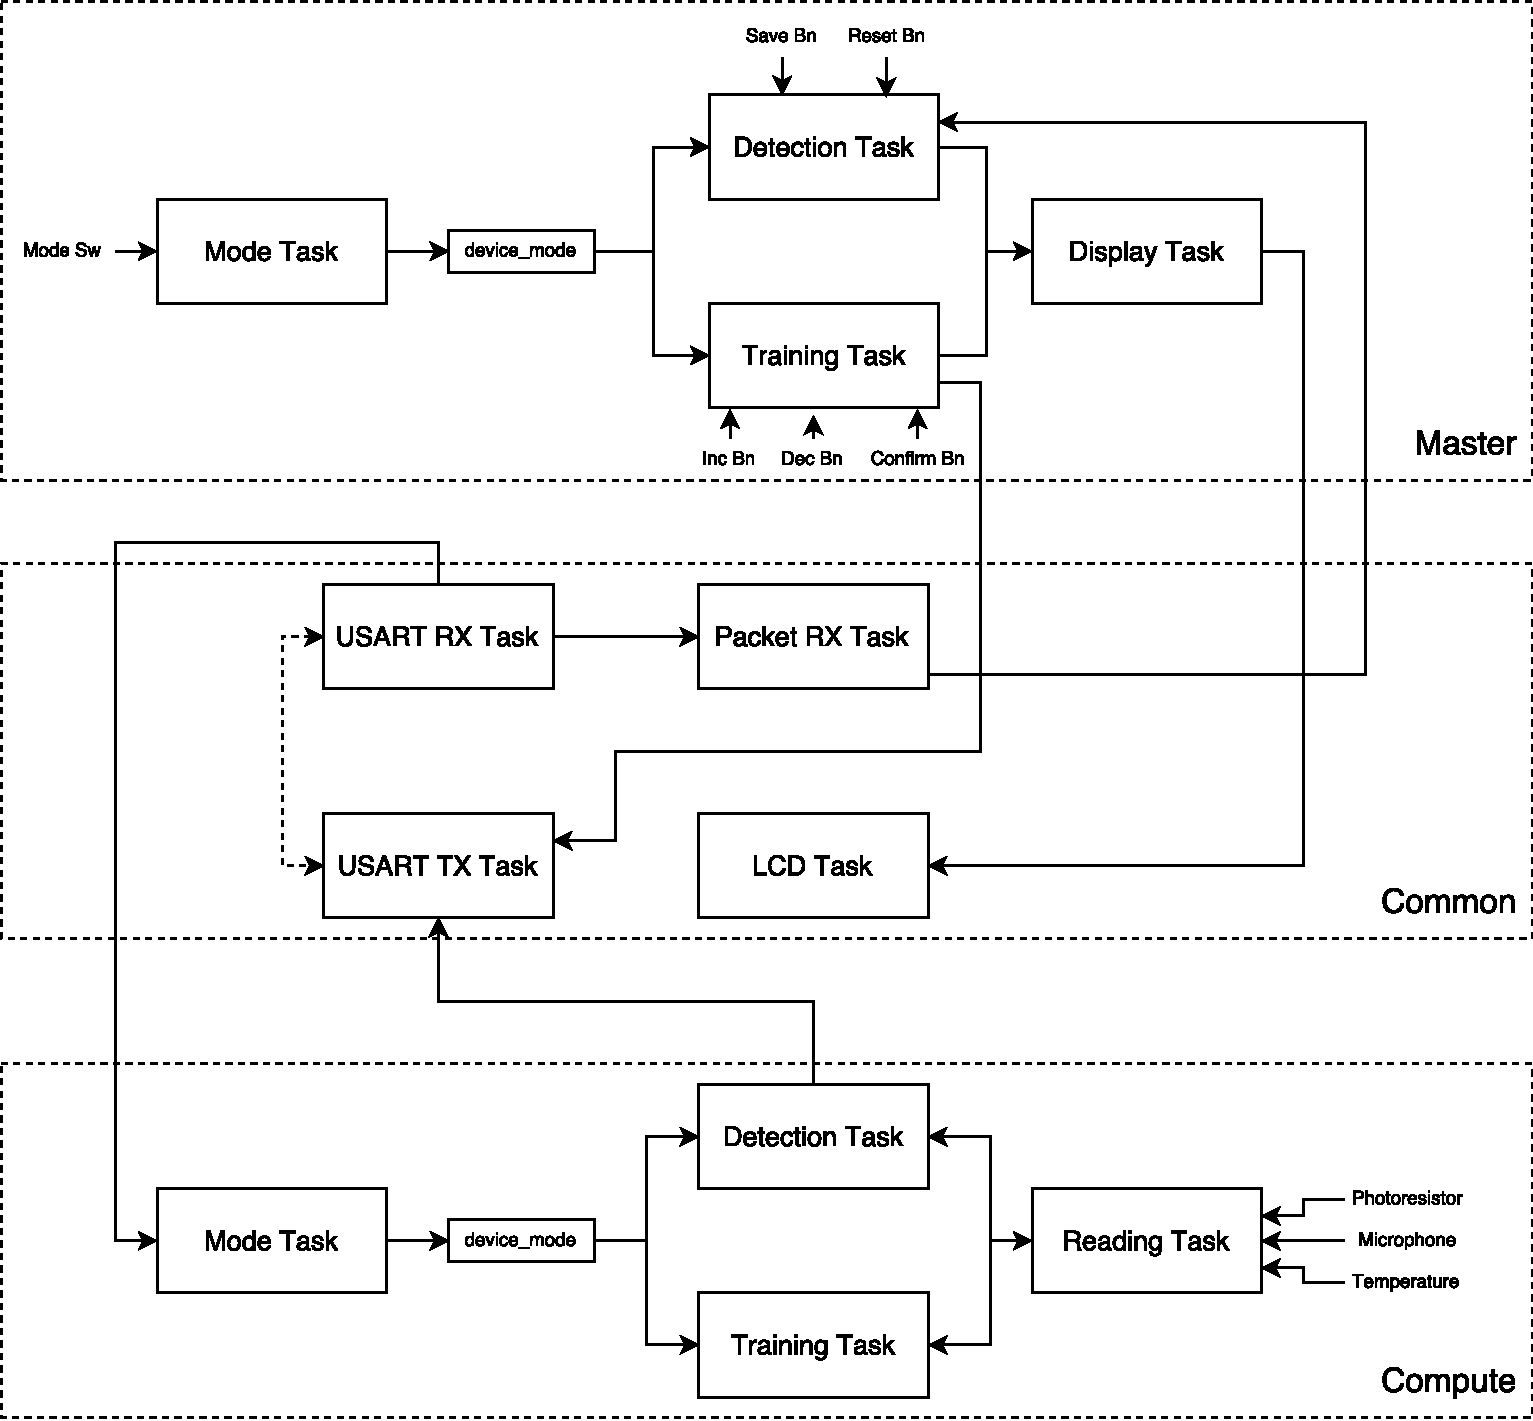
\includegraphics[width = \textwidth]{task_diagram}
  \caption{Task diagram for project}
  \label{task:1}
\end{figure}

The master and compute tasks run on their respective microcontrollers.
The common tasks run independently on both microcontrollers, being part
of a static library linked to by both microcontroller applications and
instantiated in their task schedulers.  The inputs and outputs for the
common LCD, USART TX, USART RX, and packet RX tasks were excluded from
this diagram for brevity but are documented in their task descriptions.

In the following sections, the individual tasks from the above diagram
are briefly described in addition to their inputs and outputs.  The
state machines for these tasks are presented in appendix \ref{app.sm}.

\subsection{Tasks}

\section{Complexities}

\subsection{Complete}

\begin{itemize}

  \item Using EEPROM to persist the classification model state

  \item Using USART to offload computation to a dedicated
    microcontroller

  \item Using ADC multiplexing to collect analog readings from multiple
    sensors

  \item Using a temperature sensor and microphone obtained outside of
    the lab kit

  \item Using a statistical model to perform input classification using
    fixed-point arithmetic

\end{itemize}

\subsection{Incomplete}

\begin{itemize}

  \item Using a neural network to perform input classification using
    fixed-point arithmetic \\
    This complexity could not be completed due to hardware limitations.
    Its role in the project was instead filled by the statistical model
    listed above.  The intended design for the neural network was a
    multi-layer feed-forward network, with one input layer of size 4,
    one hidden layer of size 10 with a linear activation function, one
    hidden layer of size 10 with a hyperbolic tangent activation
    function, one hidden layer of size 16 with a linear activation
    function, and one output layer of size 16 with a softmax activation
    function.  This topology was chosen as the best for fulfilling the
    goal of classifying three inputs, with one bias input, into one of
    16 outputs.  However, this network proved too large for the ATmega
    to process.  When including the amount of memory necessary for
    storing training state, the network became too large for storage in
    the ATmega's 16 kilobyte SRAM.  Additionally, even using fixed-point
    arithmetic in place of traditional floating point, the times for
    classification became slower than was considered acceptable and the
    times for training made it obvious that training would only be
    possible offline using a faster device, which was deemed to be
    beyond the scope of this project.  As a result of these limitations,
    the neural network was replaced with a simpler statistical model at
    the cost of accuracy and robustness when faced with input noise.

\end{itemize}

\section{Links}

\begin{description}

  %\item [Demonstration Video] https://youtu.be/%TODO

  \item [GitHub Repository] https://github.com/nokurn/roomdetect

\end{description}

\section{Known Issues}

\begin{itemize}

  \item The classification algorithm does not cope well with noise and
    may confuse environments with a large degree of noise as being
    equivalent regardless of the specifics of that noise.

  \item The temperature sensor is not measured with sufficient precision
    for its readings to adequately influence the results of the
    classification.

  \item The microphone primarily distinguishes between noisy and quiet
    environments with no consideration of the qualities of the sound
    such as timbre and pitch.

  \item The classifier most heavily relies on the measurements from the
    photo-resistor, despite unbiased treatment of all readings in the
    input vector.  This is likely due to the aforementioned reasons:
    low analog precision and the need for pre-processing of some
    readings.

\end{itemize}

\section{Future Work}

\begin{itemize}

  \item The largest improvement might come from replacing the compute
    microcontroller with a higher-power compute unit, possibly
    integrating floating-point arithmetic, and using a more robust
    classification model such as a neural network.

  \item By using an external analog-digital converter with higher
    precision, or simply replacing the ATmega with a microcontroller
    with a higher-precision integrated ADC, sensors with small output
    ranges would contribute more to the accuracy and confidence of the
    device's classifications.  This would reflect immediately in the
    ability of the device to distinguish between environments with
    slightly different temperatures.

  \item Applying a Fourier transform to the microphone signal and using
    the individual components as input to the classifier would improve
    the quality of classifications with regard to environmental sounds.
    For example, if one room contains several computers with spinning
    fans and another room has a single ceiling fan, yet the volume level
    in both rooms is similar, a Fourier analysis of the sound waves
    would enable the classifier to distinguish between the two by the
    timbre and pitch of the sound in addition to its loudness.

  \item Adding additional sensors would increase the size of the
    classifier's feature vector and its accuracy.  Barometric pressure,
    humidity, altitude, or even GPS would be likely candidates for
    inclusion in the system.

\end{itemize}

\appendix

\section{Appendix: State Machines}
\label{app.sm}

\subsection{Master Microcontroller}
\label{app.sm.master}

\begin{figure}[H]
  \centering
  \caption{State machine for master mode task}
  \begin{flushleft}
  \begin{description}
    \item [Input]
      \verb#PA0#
    \item [Output]
      \verb#device_mode: enum#
    \item [Period] 16 ms
  \end{description}
\end{flushleft}

\iftoggle{TASKSPECONLY}{}
{
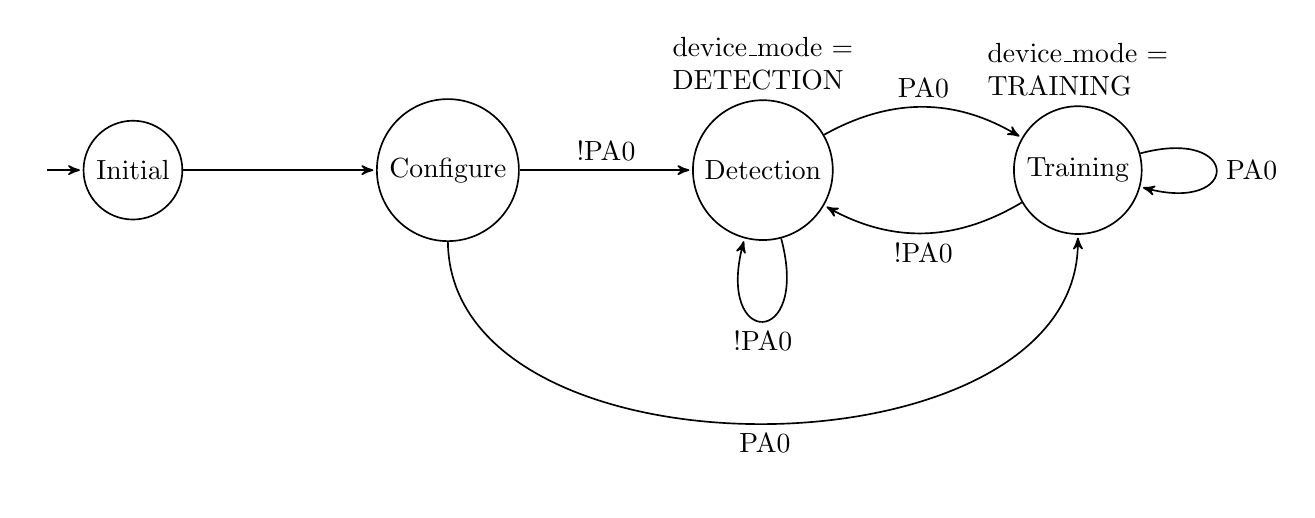
\begin{tikzpicture}[->,>=stealth',
    shorten >=1pt,
    node distance=40mm,
    auto,
    on grid,
    semithick]

  \node[state,initial]
    (Initial) {Initial};
  \node[state]
    (Configure) [right=of Initial] {Configure};
  \node[state,label={[align=left]above:{device\_mode =\\DETECTION}}]
    (Detection) [right=of Configure] {Detection};
  \node[state,label={[align=left]above:{device\_mode =\\TRAINING}}]
    (Training) [right=of Detection] {Training};

  \path[->]
    (Initial)   edge node {}     (Configure)
    (Configure) edge node {!PA0} (Detection)
    (Configure) edge [bend right=90] node [below] {PA0}  (Training)
    (Detection) edge [loop below] node {!PA0} (Detection)
    (Detection) edge [bend left] node {PA0}  (Training)
    (Training)  edge [bend left] node {!PA0} (Detection)
    (Training)  edge [loop right] node {PA0}  (Training);

\end{tikzpicture}
}

  \label{sm:1}
\end{figure}

\begin{figure}[H]
  \centering
  \caption{State machine for master detection task}
  \begin{flushleft}
  \begin{description}
    \item [Input]
      \verb#device_mode#;
      \verb#PA2#;
      \verb#PA3#
    \item [Output]
      \verb#detected_room: uint8#;
      \verb#usart_tx_queue#
    \item [Local]
      \verb#tick_count: uint16#
  \end{description}
\end{flushleft}

\iftoggle{TASKSPECONLY}{}
{
\begin{center}
  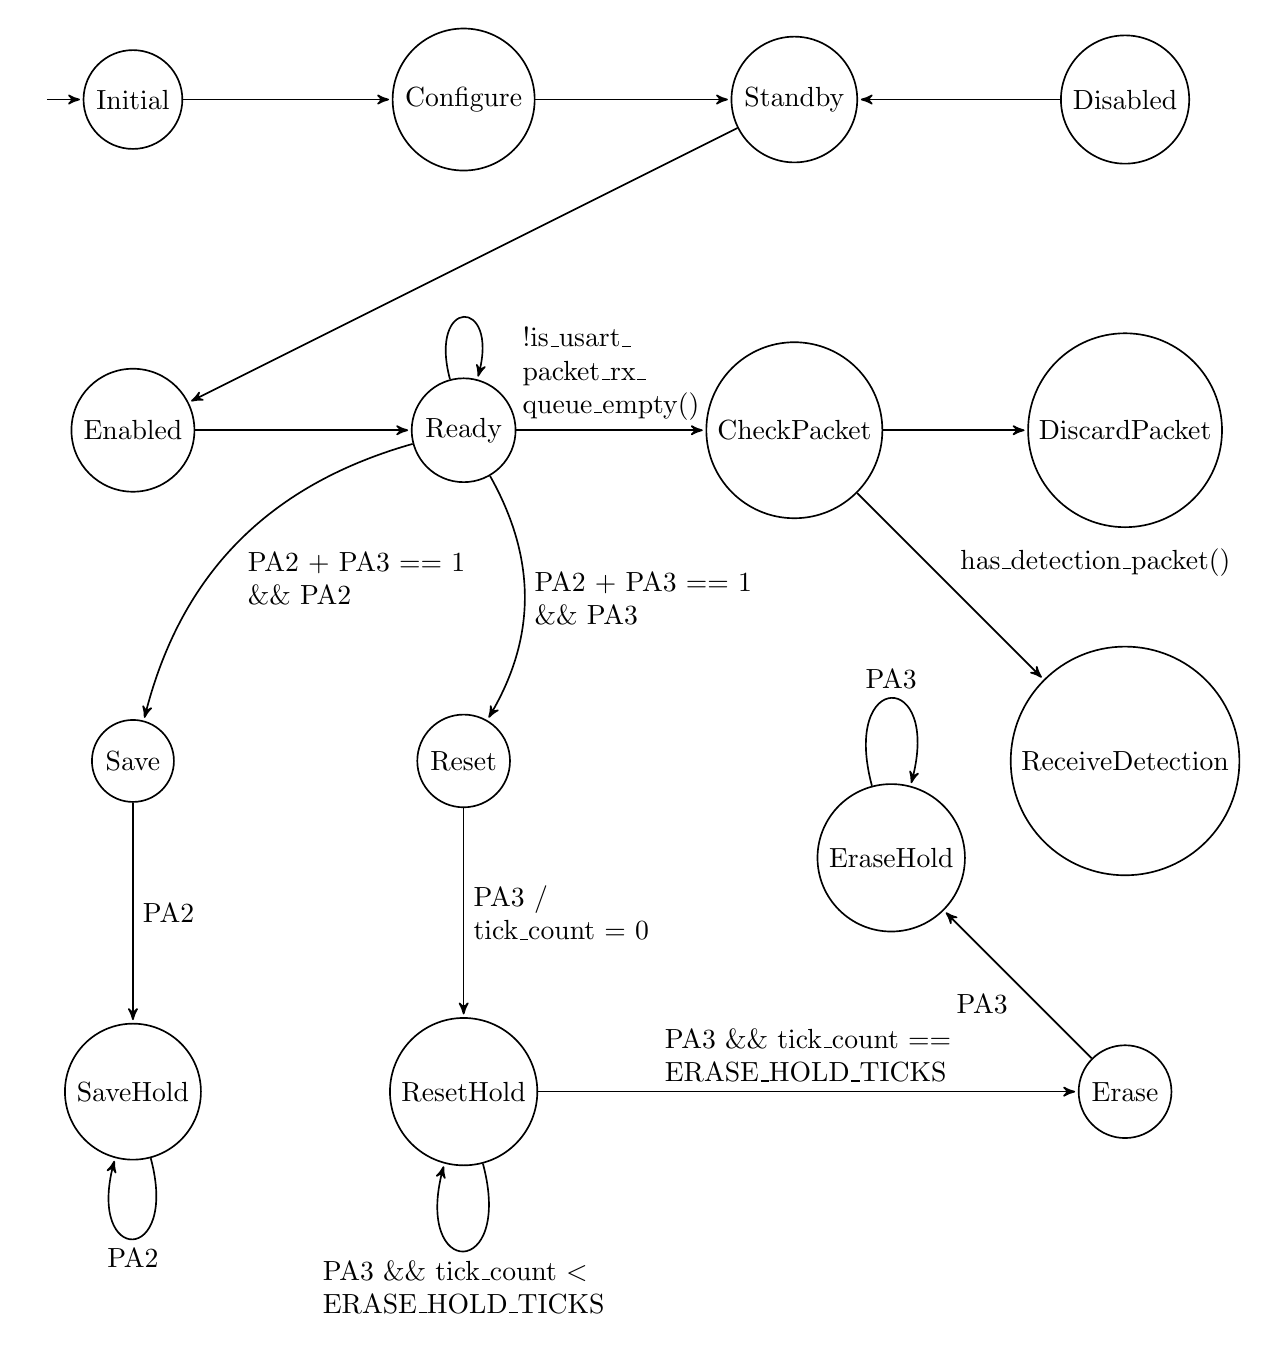
\begin{tikzpicture}[->,>=stealth',
      shorten >=1pt,
      node distance=42mm,
      auto,
      on grid,
      semithick]

    \node[state,initial]
      (Initial) {Initial};
    \node[state]
      (Configure) [right=of Initial] {Configure};
    \node[state]
      (Standby) [right=of Configure] {Standby};
    \node[state]
      (Disabled) [right=of Standby] {Disabled};
    \node[state]
      (Enabled) [below=of Initial] {Enabled};
    \node[state]
      (Ready) [right=of Enabled] {Ready};
    \node[state]
      (Reset) [below=of Ready] {Reset};
    \node[state]
      (ResetHold) [below=of Reset] {ResetHold};
    \node[state]
      (Save) [left=of Reset] {Save};
    \node[state]
      (SaveHold) [below=of Save] {SaveHold};
    \node[state]
      (CheckPacket) [right=of Ready] {CheckPacket};
    \node[state]
      (DiscardPacket) [right=of CheckPacket] {DiscardPacket};
    \node[state]
      (ReceiveDetection) [below=of DiscardPacket] {ReceiveDetection};
    \node[state]
      (Erase) [below=of ReceiveDetection] {Erase};
    \node[state]
      (EraseHold) [above left=of Erase] {EraseHold};

    \path[->]
      (Initial) edge node {} (Configure)
      (Configure) edge node {} (Standby)
      (Disabled) edge node {} (Standby)
      (Standby) edge node {} (Enabled)
      (Enabled) edge node {} (Ready)
      (Ready) edge [bend right, align = left] node {PA2 + PA3 == 1\\\&\& PA2} (Save)
      (Ready) edge [bend left, align = left] node {PA2 + PA3 == 1\\\&\& PA3} (Reset)
      (Ready) edge [align = left] node {!is\_usart\_\\packet\_rx\_\\queue\_empty()} (CheckPacket)
      (Ready) edge [loop above] node {} (Ready)
      (Save) edge node {PA2} (SaveHold)
      (SaveHold) edge [loop below] node {PA2} (SaveHold)
      (Reset) edge [align = left] node {PA3 /\\tick\_count = 0} (ResetHold)
      (ResetHold) edge [align = left] node {PA3 \&\& tick\_count ==\\ERASE\_HOLD\_TICKS} (Erase)
      (ResetHold) edge [loop below, align = left] node {PA3 \&\& tick\_count $<$\\ERASE\_HOLD\_TICKS} (ResetHold)
      (Erase) edge node {PA3} (EraseHold)
      (EraseHold) edge [loop above] node {PA3} (EraseHold)
      (CheckPacket) edge node {has\_detection\_packet()} (ReceiveDetection)
      (CheckPacket) edge node {} (DiscardPacket);

  \end{tikzpicture}
\end{center}

The following transitions have been omitted for clarity: from all states
to the Disabled state, under the condition that device\_mode !=
DETECTION; and the else-transitions from the DiscardPacket,
ReceiveDetection, Save, Reset, Erase, SaveHold, ResetHold, and EraseHold
states to the Ready state.

}

  \label{sm:2}
\end{figure}

\begin{figure}[H]
  \centering
  \caption{State machine for master training task}
  \begin{flushleft}
  \begin{description}
    \item [Input]
      \verb#device_mode#;
      \verb#PA1#;
      \verb#PA2#;
      \verb#PA3#
    \item [Output]
      \verb#training_room: uint8#;
      \verb#is_training: bool#;
      \verb#usart_tx_queue#
    \item [Local]
      \verb#tick_count: uint16#
    \item [Period] 20 ms
  \end{description}
\end{flushleft}

\iftoggle{TASKSPECONLY}{}
{
\begin{center}
  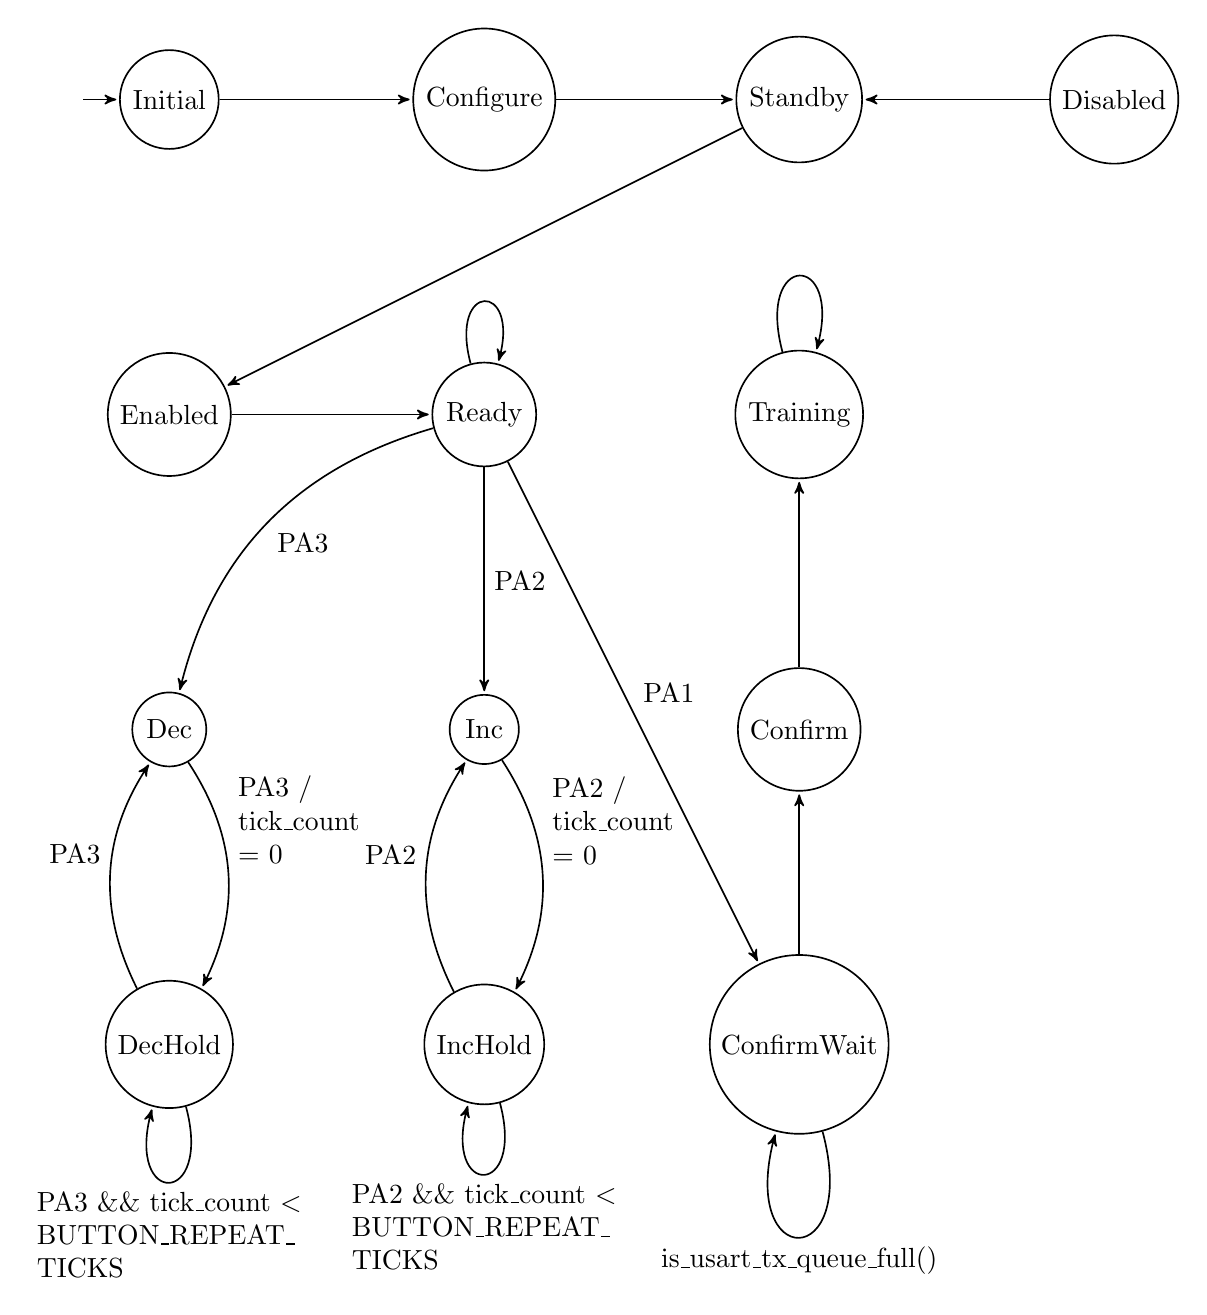
\begin{tikzpicture}[->,>=stealth',
      shorten >=1pt,
      node distance=40mm,
      auto,
      on grid,
      semithick]

    \node[state,initial]
      (Initial) {Initial};
    \node[state]
      (Configure) [right=of Initial] {Configure};
    \node[state]
      (Standby) [right=of Configure] {Standby};
    \node[state]
      (Disabled) [right=of Standby] {Disabled};
    \node[state]
      (Enabled) [below=of Initial] {Enabled};
    \node[state]
      (Ready) [right=of Enabled] {Ready};
    \node[state]
      (Inc) [below=of Ready] {Inc};
    \node[state]
      (IncHold) [below=of Inc] {IncHold};
    \node[state]
      (Dec) [left=of Inc] {Dec};
    \node[state]
      (DecHold) [below=of Dec] {DecHold};
    \node[state]
      (Training) [right=of Ready] {Training};
    \node[state]
      (Confirm) [below=of Training] {Confirm};
    \node[state]
      (ConfirmWait) [below=of Confirm] {ConfirmWait};

    \path[->]
      (Initial) edge node {} (Configure)
      (Configure) edge node {} (Standby)
      (Disabled) edge node {} (Standby)
      (Standby) edge node {} (Enabled)
      (Enabled) edge node {} (Ready)
      (Ready) edge [bend right, align = left] node {PA3} (Dec)
      (Ready) edge [align = left] node {PA2} (Inc)
      (Ready) edge [align = left] node {PA1} (ConfirmWait)
      (Ready) edge [loop above] node {} (Ready)
      (Inc) edge [bend left, align = left] node {PA2 /\\tick\_count\\= 0} (IncHold)
      (IncHold) edge [bend left, align = left] node {PA2} (Inc)
      (IncHold) edge [loop below, align = left] node {PA2 \&\& tick\_count $<$\\BUTTON\_REPEAT\_\\TICKS} (IncHold)
      (Dec) edge [bend left, align = left] node {PA3 /\\tick\_count\\= 0} (DecHold)
      (DecHold) edge [bend left, align = left] node {PA3} (Dec)
      (DecHold) edge [loop below, align = left] node {PA3 \&\& tick\_count $<$\\BUTTON\_REPEAT\_\\TICKS} (DecHold)
      (ConfirmWait) edge [loop below] node {is\_usart\_tx\_queue\_full()} (ConfirmWait)
      (ConfirmWait) edge node {} (Confirm)
      (Confirm) edge node {} (Training)
      (Training) edge [loop above] node {} (Training);

  \end{tikzpicture}
\end{center}

The following transitions have been omitted for clarity: from all states
to the Disabled state, under the condition that device\_mode !=
TRAINING; and the else-transitions from the Inc, IncHold, Dec, and
DecHold states to the Ready state.  The transition conditions from the
Ready state to the Dec, Inc, and ConfirmWait states are also conjoined
with the condition that PA1 + PA2 + PA3 == 1.  The transition conditions
from the DecHold and IncHold states to the Dec and Inc states,
respectively, are also conjoined with the condition that tick\_count ==
BUTTON\_REPEAT\_TICKS.

}

  \label{sm:3}
\end{figure}

\begin{figure}[H]
  \centering
  \caption{State machine for master display task}
  \begin{flushleft}
  \begin{description}
    \item [Input]
      \verb#detected_room#;
      \verb#training_room#;
      \verb#is_training#;
      \verb#should_display_save#;
      \verb#should_display_reset#;
      \verb#should_display_erase#;
      \verb#is_lcd_ready#
    \item [Output]
      \verb#should_lcd_clear#;
      \verb#should_lcd_write#;
      \verb#lcd_buffer#;
      \verb#lcd_position#
    \item [Local]
      \verb#last_room: uint8#
    \item [Period] 20 ms
  \end{description}
\end{flushleft}

\iftoggle{TASKSPECONLY}{}
{
\begin{center}
  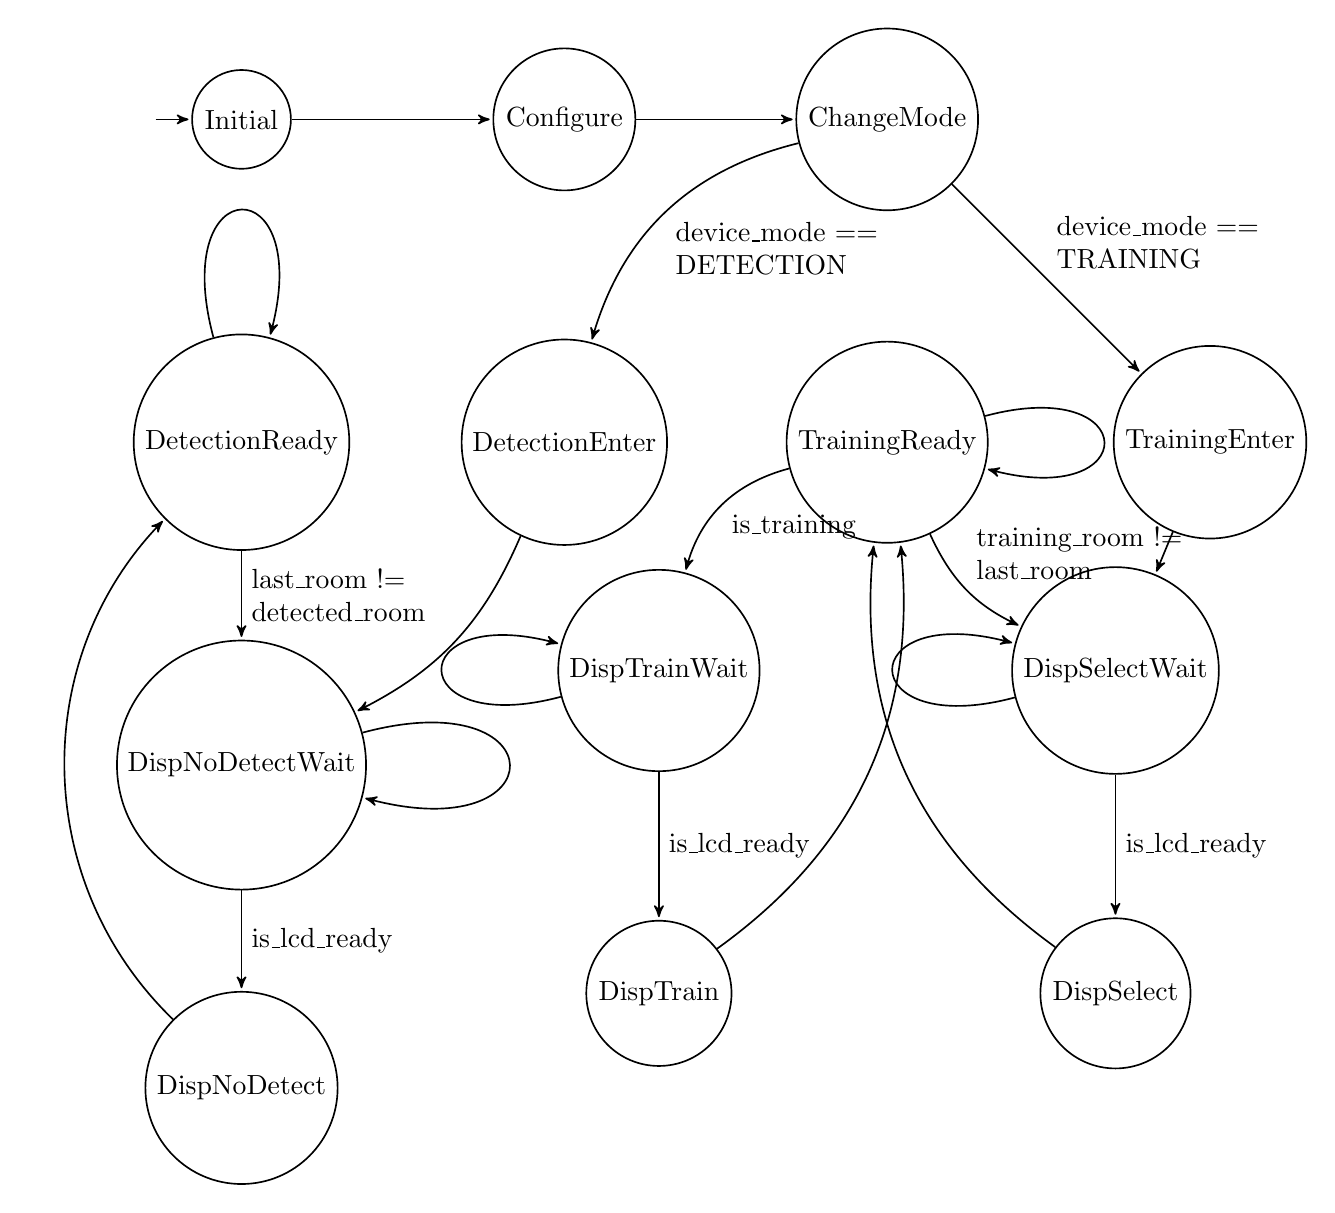
\begin{tikzpicture}[->,>=stealth',
      shorten >=1pt,
      node distance=41mm,
      auto,
      on grid,
      semithick]

    \node[state,initial]
      (Initial) {Initial};
    \node[state]
      (Configure) [right=of Initial] {Configure};
    \node[state]
      (ChangeMode) [right=of Configure] {ChangeMode};
    \node[state]
      (DetectionEnter) [below=of Configure] {DetectionEnter};
    \node[state]
      (DetectionReady) [left=of DetectionEnter] {DetectionReady};
    \node[state]
      (DispNoDetectWait) [below=of DetectionReady] {DispNoDetectWait};
    \node[state]
      (DispNoDetect) [below=of DispNoDetectWait] {DispNoDetect};
    \node[state]
      (TrainingReady) [below=of ChangeMode] {TrainingReady};
    \node[state]
      (TrainingEnter) [right=of TrainingReady] {TrainingEnter};
    \node[state]
      (DispSelectWait) [below right of=TrainingReady] {DispSelectWait};
    \node[state]
      (DispSelect) [below of=DispSelectWait] {DispSelect};
    \node[state]
      (DispTrainWait) [below left of=TrainingReady] {DispTrainWait};
    \node[state]
      (DispTrain) [below of=DispTrainWait] {DispTrain};

    \path[->]
      (Initial) edge node {} (Configure)
      (Configure) edge node {} (ChangeMode)
      (ChangeMode) edge [bend right, align=left] node {device\_mode ==\\DETECTION} (DetectionEnter)
      (ChangeMode) edge [align=left] node {device\_mode ==\\TRAINING} (TrainingEnter)
      (DetectionEnter) edge [bend left=20] node {} (DispNoDetectWait)
      (DetectionReady) edge [align=left] node {last\_room !=\\detected\_room} (DispNoDetectWait)
      (DetectionReady) edge [loop above] node {} (DetectionReady)
      (DispNoDetect) edge [bend left=45] node {} (DetectionReady)
      (DispNoDetectWait) edge node {is\_lcd\_ready} (DispNoDetect)
      (DispNoDetectWait) edge [loop right] node {} (DispNoDetectWait)
      (TrainingEnter) edge node {} (DispSelectWait)
      (TrainingReady) edge [bend right=20, align=left] node {training\_room !=\\last\_room} (DispSelectWait)
      (TrainingReady) edge [bend right=30, align=left] node {is\_training} (DispTrainWait)
      (TrainingReady) edge [loop right] node {} (TrainingReady)
      (DispSelect) edge [bend left] node {} (TrainingReady)
      (DispSelectWait) edge node {is\_lcd\_ready} (DispSelect)
      (DispSelectWait) edge [loop left] (DispSelectWait)
      (DispTrain) edge [bend right] node {} (TrainingReady)
      (DispTrainWait) edge node {is\_lcd\_ready} (DispTrain)
      (DispTrainWait) edge [loop left] (DispTrainWait);

  \end{tikzpicture}
\end{center}

The following transitions have been omitted for clarity: from all states
to the ChangeMode state, under the condition that device\_mode is
different from the expected mode for the given state.  The
DispNoDetectWait and DispNoDetect states are duplicated, including
transitions, for the following similar states: Detect, Save, Reset, and
Erase.  These redundant states have been omitted for clarity.

}

  \label{sm:4}
\end{figure}

\subsection{Compute Microcontroller}
\label{app.sm.compute}

\begin{figure}[H]
  \centering
  \caption{State machine for compute mode task}
  \begin{flushleft}
  \begin{description}
    \item [Input]
      \verb#usart_packet_rx_queue#
    \item [Output]
      \verb#device_mode: enum#;
      \verb#training_room: uint8#
  \end{description}
\end{flushleft}

\iftoggle{TASKSPECONLY}{}
{
\begin{center}
  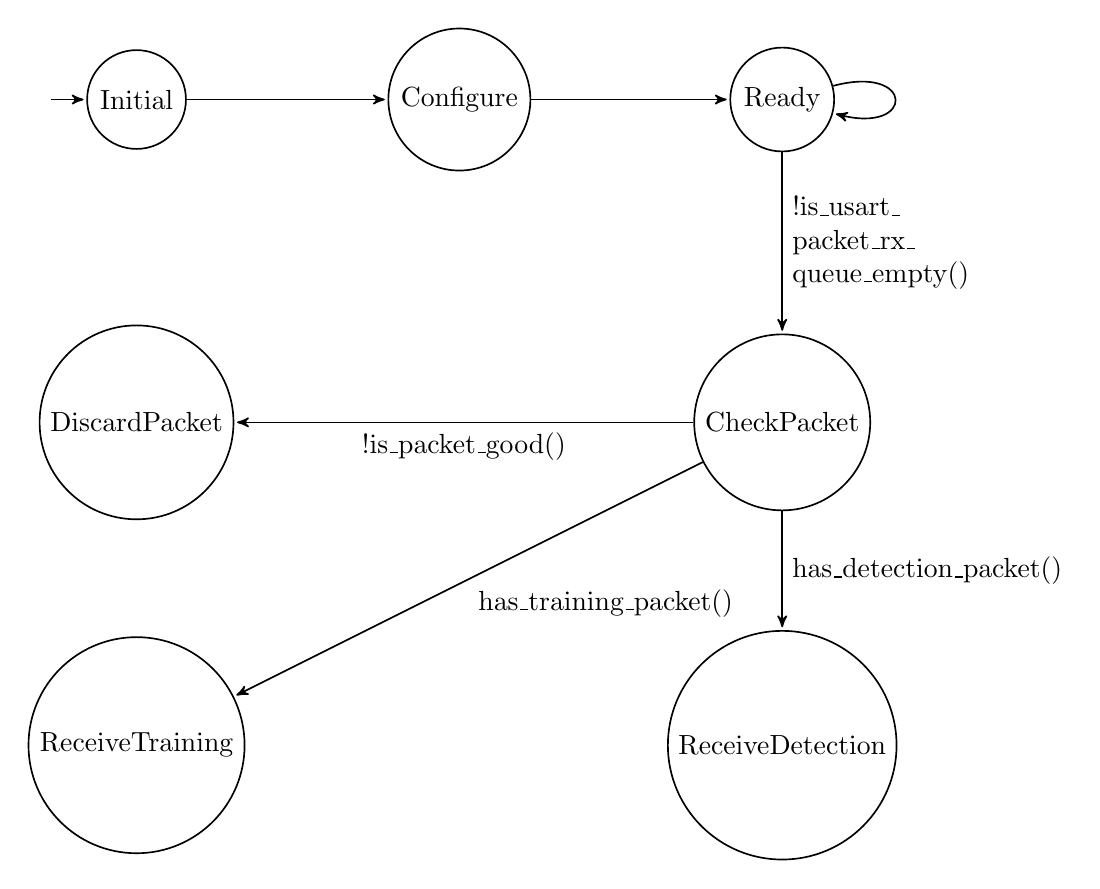
\begin{tikzpicture}[->,>=stealth',
      shorten >=1pt,
      node distance=41mm,
      auto,
      on grid,
      semithick]

    \node[state,initial]
      (Initial) {Initial};
    \node[state]
      (Configure) [right=of Initial] {Configure};
    \node[state]
      (Ready) [right=of Configure] {Ready};
    \node[state]
      (CheckPacket) [below of=Ready] {CheckPacket};
    \node[state]
      (DiscardPacket) [below of=Initial] {DiscardPacket};
    \node[state]
      (ReceiveDetection) [below of=CheckPacket] {ReceiveDetection};
    \node[state]
      (ReceiveTraining) [below of=DiscardPacket] {ReceiveTraining};

    \path[->]
      (Initial) edge node {} (Configure)
      (Configure) edge node {} (Ready)
      (Ready) edge [align=left] node {!is\_usart\_\\packet\_rx\_\\queue\_empty()} (CheckPacket)
      (Ready) edge [loop right] node {} (Ready)
      (CheckPacket) edge node {!is\_packet\_good()} (DiscardPacket)
      (CheckPacket) edge node {has\_detection\_packet()} (ReceiveDetection)
      (CheckPacket) edge node {has\_training\_packet()} (ReceiveTraining);

  \end{tikzpicture}
\end{center}

The following transitions have been omitted for clarity: from the
DiscardPacket, ReceiveDetection, and ReceiveTraining states to the Ready
state under any condition.

}

  \label{sm:5}
\end{figure}

\begin{figure}[H]
  \centering
  \caption{State machine for compute reading task}
  \begin{flushleft}
  \begin{description}
    \item [Input]
      \verb#should_poll_readings: bool#;
      \verb#adc#
    \item [Output]
      \verb#reading_vector: accum[]#;
      \verb#are_readings_ready: bool#
    \item [Local]
      \verb#readings: accum[]#;
      \verb#index: size#;
      \verb#samples: size#
  \end{description}
\end{flushleft}

\iftoggle{TASKSPECONLY}{}
{
\begin{center}
  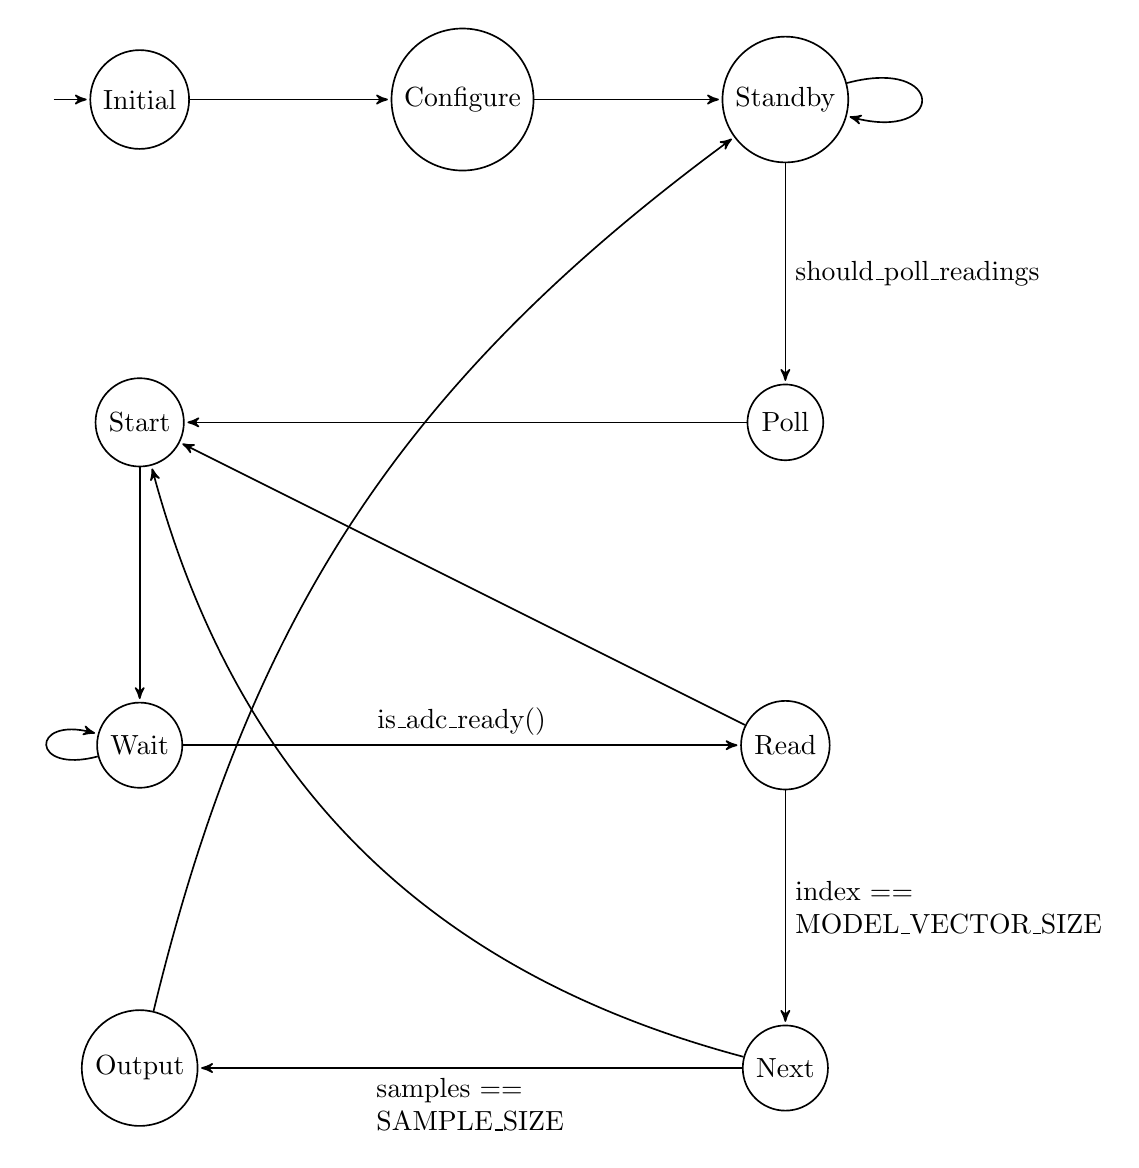
\begin{tikzpicture}[->,>=stealth',
      shorten >=1pt,
      node distance=41mm,
      auto,
      on grid,
      semithick]

    \node[state,initial]
      (Initial) {Initial};
    \node[state]
      (Configure) [right=of Initial] {Configure};
    \node[state]
      (Standby) [right=of Configure] {Standby};
    \node[state]
      (Poll) [below of=Standby] {Poll};
    \node[state]
      (Start) [below of=Initial] {Start};
    \node[state]
      (Wait) [below of=Start] {Wait};
    \node[state]
      (Read) [below of=Poll] {Read};
    \node[state]
      (Next) [below of=Read] {Next};
    \node[state]
      (Output) [below of=Wait] {Output};

    \path[->]
      (Initial) edge node {} (Configure)
      (Configure) edge node {} (Standby)
      (Standby) edge node {should\_poll\_readings} (Poll)
      (Standby) edge [loop right] node {} (Standby)
      (Poll) edge node {} (Start)
      (Start) edge node {} (Wait)
      (Wait) edge node {is\_adc\_ready()} (Read)
      (Wait) edge [loop left] node {} (Wait)
      (Read) edge [align=left] node {index ==\\MODEL\_VECTOR\_SIZE} (Next)
      (Read) edge node {} (Start)
      (Next) edge [align=left] node {samples ==\\SAMPLE\_SIZE} (Output)
      (Next) edge [bend left] node {} (Start)
      (Output) edge [bend left=20] node {} (Standby);

  \end{tikzpicture}
\end{center}

}

  \label{sm:6}
\end{figure}

\begin{figure}[H]
  \centering
  \caption{State machine for compute detection task}
  \begin{flushleft}
  \begin{description}
    \item [Input]
      \verb#device_mode#;
      \verb#reading_vector#;
      \verb#are_readings_ready#
    \item [Output]
      \verb#detected_room: uint8#;
      \verb#should_poll_readings#
  \end{description}
\end{flushleft}

\iftoggle{TASKSPECONLY}{}
{
\begin{center}
  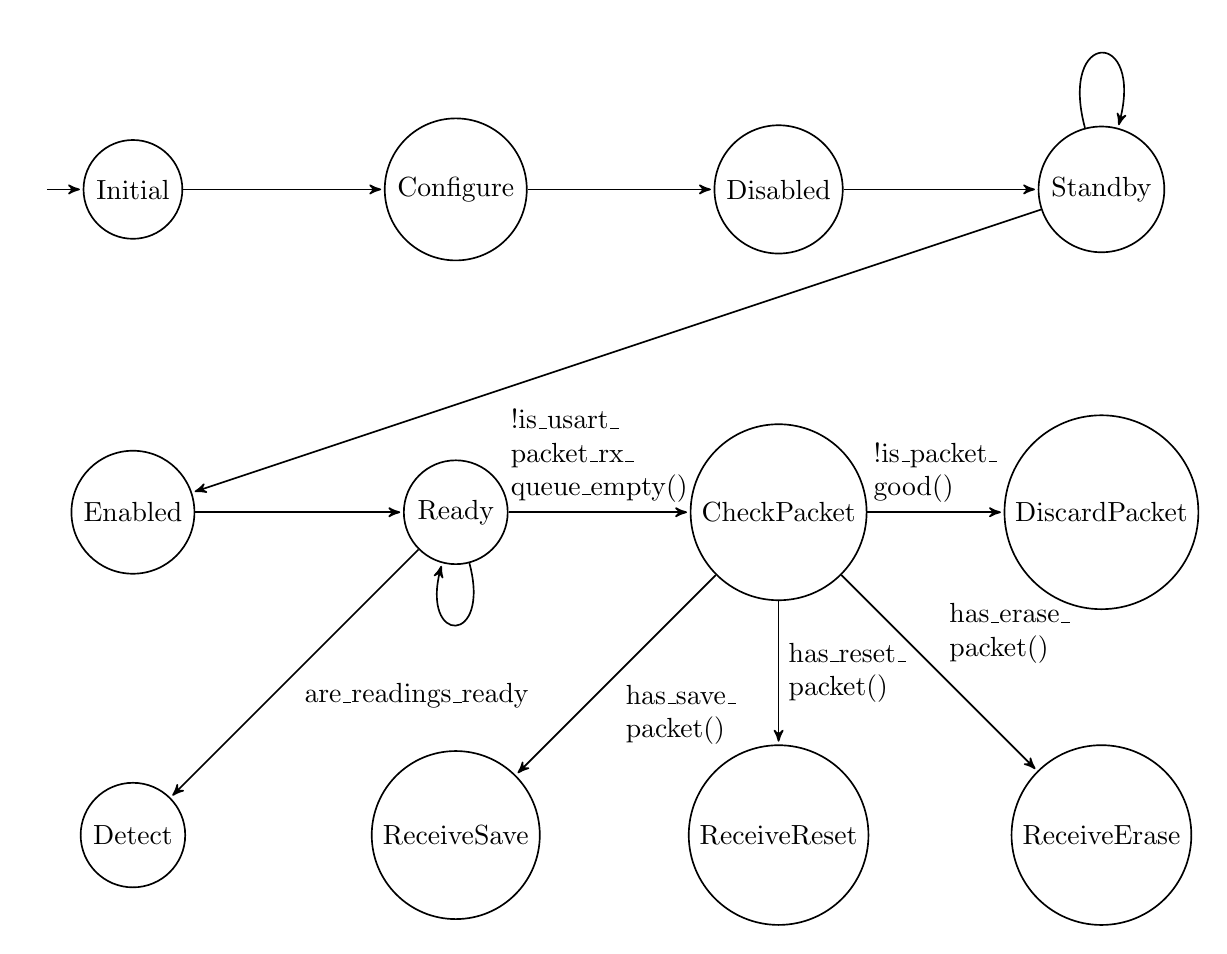
\begin{tikzpicture}[->,>=stealth',
      shorten >=1pt,
      node distance=41mm,
      auto,
      on grid,
      semithick]

    \node[state,initial]
      (Initial) {Initial};
    \node[state]
      (Configure) [right=of Initial] {Configure};
    \node[state]
      (Disabled) [right=of Configure] {Disabled};
    \node[state]
      (Standby) [right=of Disabled] {Standby};
    \node[state]
      (Enabled) [below of=Initial] {Enabled};
    \node[state]
      (Ready) [right of=Enabled] {Ready};
    \node[state]
      (Detect) [below of=Enabled] {Detect};
    \node[state]
      (CheckPacket) [right of=Ready] {CheckPacket};
    \node[state]
      (DiscardPacket) [right of=CheckPacket] {DiscardPacket};
    \node[state]
      (ReceiveReset) [below of=CheckPacket] {ReceiveReset};
    \node[state]
      (ReceiveSave) [left of=ReceiveReset] {ReceiveSave};
    \node[state]
      (ReceiveErase) [right of=ReceiveReset] {ReceiveErase};

    \path[->]
      (Initial) edge node {} (Configure)
      (Configure) edge node {} (Disabled)
      (Disabled) edge node {} (Standby)
      (Standby) edge [loop above] node {} (Standby)
      (Standby) edge node {} (Enabled)
      (Enabled) edge node {} (Ready)
      (Ready) edge [align=left] node {!is\_usart\_\\packet\_rx\_\\queue\_empty()} (CheckPacket)
      (Ready) edge node {are\_readings\_ready} (Detect)
      (Ready) edge [loop below] node {} (Ready)
      (CheckPacket) edge [align=left] node {!is\_packet\_\\good()} (DiscardPacket)
      (CheckPacket) edge [align=left] node {has\_save\_\\packet()} (ReceiveSave)
      (CheckPacket) edge [align=left] node {has\_reset\_\\packet()} (ReceiveReset)
      (CheckPacket) edge [align=left] node {has\_erase\_\\packet()} (ReceiveErase);

  \end{tikzpicture}
\end{center}

The following transitions have been omitted for clarity: from the
Detect, DiscardPacket, ReceiveSave, ReceiveReset, and ReceiveErase
states to the Ready state under any condition; the else-transition from
the CheckPacket state to the Ready state; and from all states to the
Disabled state when device\_mode != DETECTION.

}

  \label{sm:7}
\end{figure}

\begin{figure}[H]
  \centering
  \caption{State machine for compute training task}
  \begin{flushleft}
  \begin{description}
    \item [Input]
      \verb#device_mode#;
      \verb#reading_vector#;
      \verb#are_readings_ready#;
      \verb#training_room: uint8#
    \item [Output]
      \verb#should_poll_readings#
  \end{description}
\end{flushleft}

\iftoggle{TASKSPECONLY}{}
{
\begin{center}
  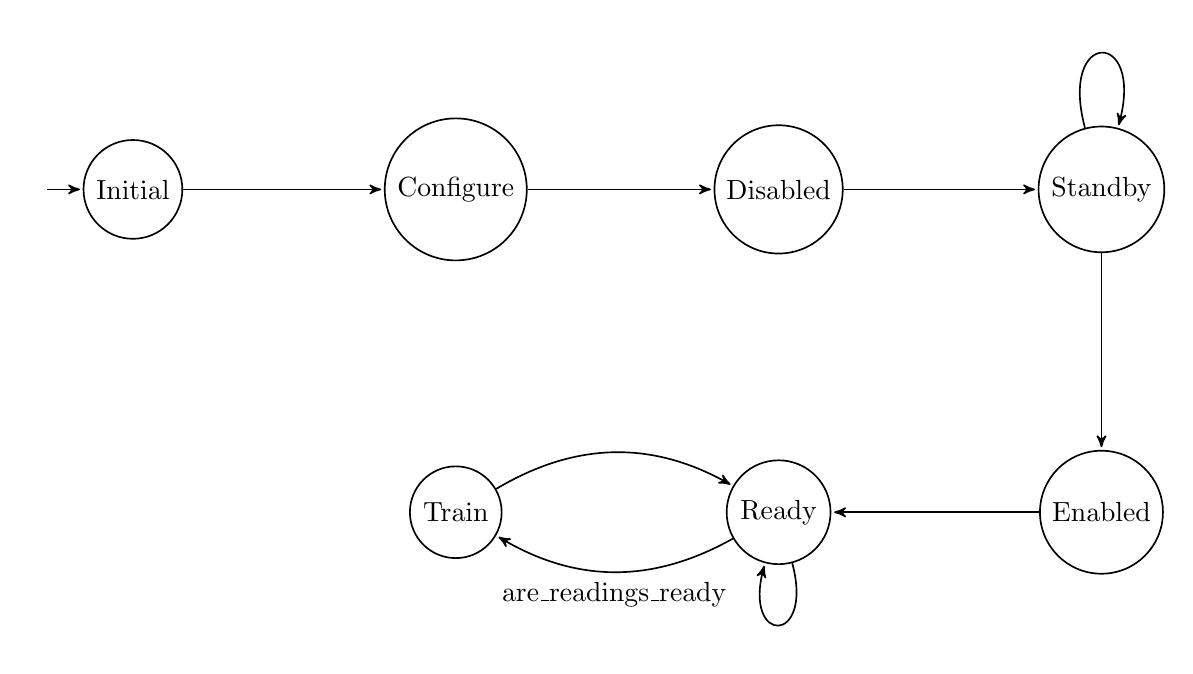
\begin{tikzpicture}[->,>=stealth',
      shorten >=1pt,
      node distance=41mm,
      auto,
      on grid,
      semithick]

    \node[state,initial]
      (Initial) {Initial};
    \node[state]
      (Configure) [right=of Initial] {Configure};
    \node[state]
      (Disabled) [right=of Configure] {Disabled};
    \node[state]
      (Standby) [right=of Disabled] {Standby};
    \node[state]
      (Enabled) [below of=Standby] {Enabled};
    \node[state]
      (Ready) [left of=Enabled] {Ready};
    \node[state]
      (Train) [left of=Ready] {Train};

    \path[->]
      (Initial) edge node {} (Configure)
      (Configure) edge node {} (Disabled)
      (Disabled) edge node {} (Standby)
      (Standby) edge [loop above] node {} (Standby)
      (Standby) edge node {} (Enabled)
      (Enabled) edge node {} (Ready)
      (Ready) edge [bend left] node {are\_readings\_ready} (Train)
      (Ready) edge [loop below] node {} (Ready)
      (Train) edge [bend left] node {} (Ready);

  \end{tikzpicture}
\end{center}

The following transitions have been omitted for clarity:  from all
states to the Disabled state when device\_mode != TRAINING.

}

  \label{sm:8}
\end{figure}

\subsection{Common Infrastructure}
\label{app.sm.common}

\begin{figure}[H]
  \centering
  \caption{State machine for common LCD task}
  \begin{flushleft}
  \begin{description}
    \item [Input]
      \verb#should_lcd_clear: bool#;
      \verb#should_lcd_write: bool#;
      \verb#lcd_buffer: char[]#;
      \verb#lcd_position: uint8#
    \item [Output]
      \verb#is_lcd_ready: bool#
    \item [Local]
      \verb#index: size#
  \end{description}
\end{flushleft}

  \label{sm:9}
\end{figure}

\begin{figure}[H]
  \centering
  \caption{State machine for common USART TX task}
  \begin{flushleft}
  \begin{description}
    \item [Input]
      \verb#usart_tx_queue: uint8[]#;
      \verb#usart_tx_queue_size: size#;
      \verb#usart_tx_queue_head: size#;
      \verb#usart_tx_queue_tail: size#
    \item [Output]
      \verb#usart_tx_queue#
    \item [Period] 1 ms
  \end{description}
\end{flushleft}

\iftoggle{TASKSPECONLY}{}
{
}

  \label{sm:10}
\end{figure}

\begin{figure}[H]
  \centering
  \caption{State machine for common USART RX task}
  \begin{flushleft}
  \begin{description}
    \item [Input]
      \verb#usart_rx_queue#
    \item [Output]
      \verb#usart_rx_queue: uint8[]#;
      \verb#usart_rx_queue_size: size#;
      \verb#usart_rx_queue_head: size#;
      \verb#usart_rx_queue_tail: size#
  \end{description}
\end{flushleft}

\iftoggle{TASKSPECONLY}{}
{
}

  \label{sm:11}
\end{figure}

\begin{figure}[H]
  \centering
  \caption{State machine for common USART packet RX task}
  \begin{flushleft}
  \begin{description}
    \item [Input]
      \verb#usart_rx_queue#
    \item [Output]
      \verb#usart_packet_rx_queue: usart_packet[]#;
      \verb#usart_packet_rx_queue_size: size#;
      \verb#usart_packet_rx_queue_head: size#;
      \verb#usart_packet_rx_queue_tail: size#
    \item [Period] 1 ms
  \end{description}
\end{flushleft}

\iftoggle{TASKSPECONLY}{}
{
}

  \label{sm:12}
\end{figure}

\end{document}
